\chapter{Stereoscopic Video}
\markright{Stereoscopic Video}
\label{stereo_video}
\phantomsection
%\addcontentsline{toc}{chapter}{Stereoscopic Video}

In a wide variety of image processing applications, explicit depth information is required in
addition to general image informations, such as intensities, color, densities.\\
Examples of such applications are found in 3D vision (robot vision, photogrammetry, remote sensing systems), in medical imaging (computer tomography,
magnetic resonance imaging, microsurgery), in remote handling of objects (random bin picking), in space exploration (mobile robotics navigation) or 3D movies and videogames.\\
In each of these cases, depth information is essential for accurate image analysis or for enhancing the
realism.\\
In remote sensing the terrain's elevation needs to be accurately determined for map production, in remote handling an operator needs to have precise knowledge of the threedimensional organization of the area to avoid collisions and misplacements.\\
\begin{figure}[h!]
\centering
\begin{subfigure}[]{0.5\textwidth}
		\centering
        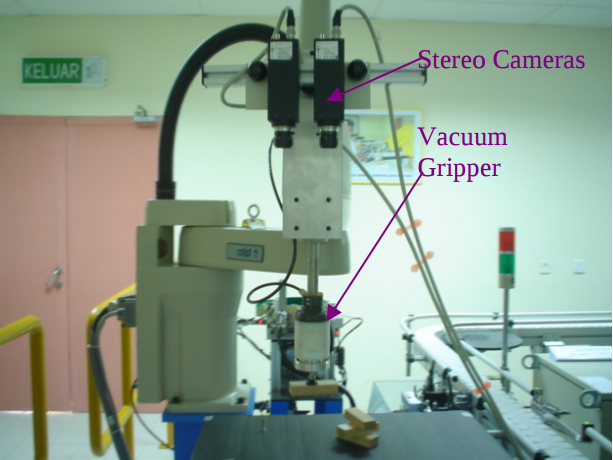
\includegraphics[width=0.7\textwidth]{./img/bin_pick.png}
                \caption{\scriptsize{In bin picking applications stereo vision helps to reconstruct the 3D environment and detect the part of the object to be robotically picked}}
\end{subfigure}% 
~ \quad
\begin{subfigure}[]{0.5\textwidth}
	\centering
	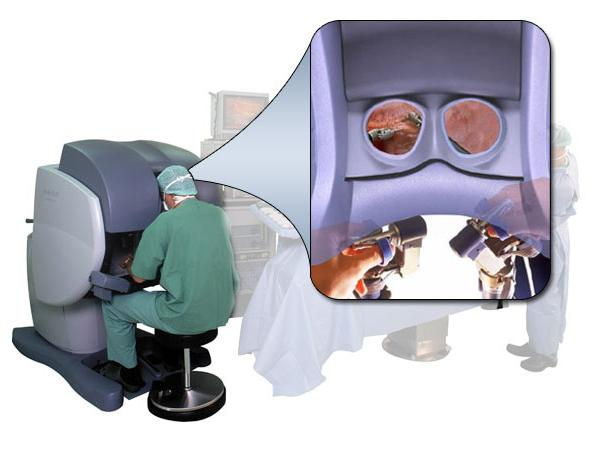
\includegraphics[width=0.7\textwidth]{./img/da_vinci.jpg}
          \caption{\scriptsize{Surgical robot \textit{Da vinci} is provided with a stereoscopic camera that allows a tridimensional view of the operative filed.}}
\end{subfigure} 
\caption{\small{Stereoscopy in medical and industrial field}}
\end{figure}

\begin{figure}[h!]
\centering
\begin{subfigure}[]{0.5\textwidth}
		\centering
        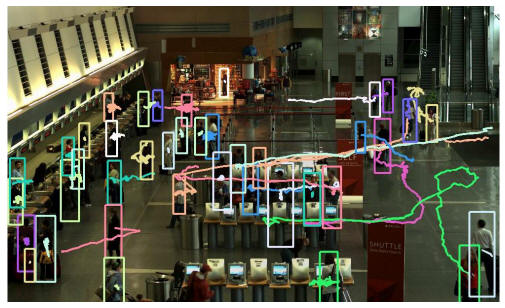
\includegraphics[width=0.7\textwidth]{./img/tracking.jpg}
                \caption{\scriptsize{In people tracking application stereo vision improves segmentation thanks to depth information and it's less sensible to light changes.}}
\end{subfigure}% 
~ \quad
\begin{subfigure}[]{0.5\textwidth}
		\centering
        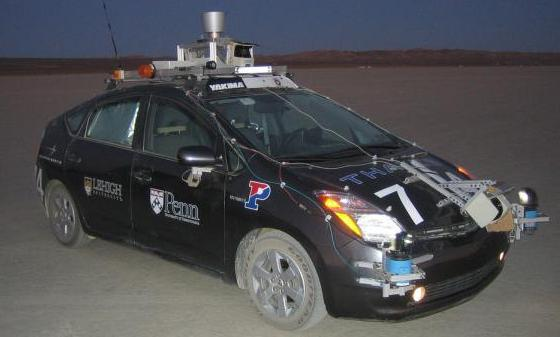
\includegraphics[width=0.7\textwidth]{./img/little_ben.jpg}
                \caption{\scriptsize{In mobile robotics navigation stereo vision has became the first choice technology because it provids a lot of quality data for low costs.}}
\end{subfigure} 
\caption{\small{Stereoscopy application's fields}}
\end{figure}
Depth in real world scenes can be explicitly measured by a number of range sensing devices such as by laser range sensors, by structured light or by ultrasound.
However it's usually undesirable to have separate systems for acquiring the intensity and the depth
information because of the relative low resolution of the range sensing devices and because it's not an easy task to fuse information from different type of sensors; for these reasons and for a non-negligible economic factor stereoscopic vision has becoming the technology of choice in these type of applications.
\begin{figure}[h!]
\centering
\begin{subfigure}[]{0.4\textwidth}
		\centering
        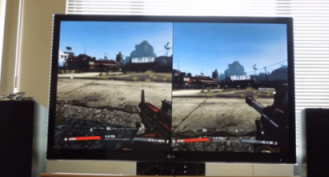
\includegraphics[width=0.7\textwidth]{./img/games1.png}
                \caption{\scriptsize{Stereo video frames, left and right.\newline}}
\end{subfigure}
\begin{subfigure}[]{0.4\textwidth}
		\centering
        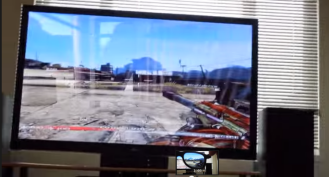
\includegraphics[width=0.7\textwidth]{./img/games2.png}
                \caption{\scriptsize{Overlap of the two frames.}}
\end{subfigure} 
\begin{subfigure}[]{0.4\textwidth}
		\centering
        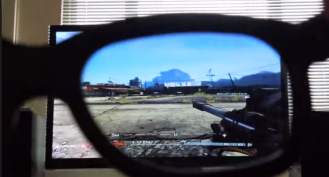
\includegraphics[width=0.7\textwidth]{./img/games3.png}
                \caption{\scriptsize{3D view with specific glasses}}
\end{subfigure}%
\begin{subfigure}[]{0.4\textwidth}
		\centering
        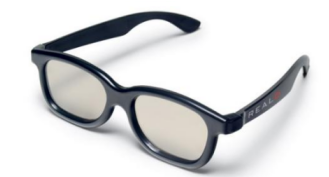
\includegraphics[width=0.7\textwidth]{./img/games4.png}
                \caption{\scriptsize{Polarized glasses for 3D view}}
\end{subfigure} 
\caption{\small{Stereoscopy in 3D video games}}
\end{figure}

\section{Stereo vision}
In image processing stereo vision is the process of extracting 3D information from multiple 2D views of a scene. \\
The 3D information can be obtained from a pair of images, also known as a stereo pair, by estimating the relative depth of points in the scene.\\
From the anatomic point of view, the human brain calculates the depth in a visual scene mainly by
processing the information brought by the images seen by the left and the right eyes. These left and right images are slightly different because the eyes have biologically different emplacements.\\
Consequently, the straightforward way of achieving stereoscopic digital imaging is to emulate the
Human Visual System (HSV) by setting-up (under controlled geometric positions), two traditional 2D
cameras.\\
\begin{figure}[h]
\centering
\begin{subfigure}[b]{0.35\textwidth}
        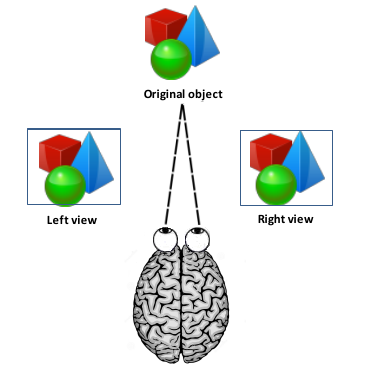
\includegraphics[width=\textwidth]{./img/hvs.png}
         \caption{\scriptsize{Binocular human visual system}}
         \label{fig:hvs}
\end{subfigure}
\begin{subfigure}[b]{0.35\textwidth}
        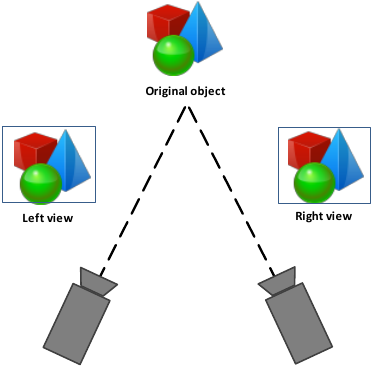
\includegraphics[width=\textwidth]{./img/stereo.png}
        \caption{\scriptsize{Stereoscopic system}}
        \label{fig:stereo}
\end{subfigure} 
\caption{\small{Binocular human vision vs. stereoscopic content acquisition.}}
\end{figure}

\subsection{Stereo Vision Geometry}

In order to be able to perceive depth using recorded images, a stereoscopic camera is required
which consists of two cameras that capture two different, horizontally shifted perspective
viewpoints; with two (or more) cameras we can infer depth, by means of triangulation, if we are able to find corresponding points in the two images (Figure).\\
\begin{figure}[h!]
\centering
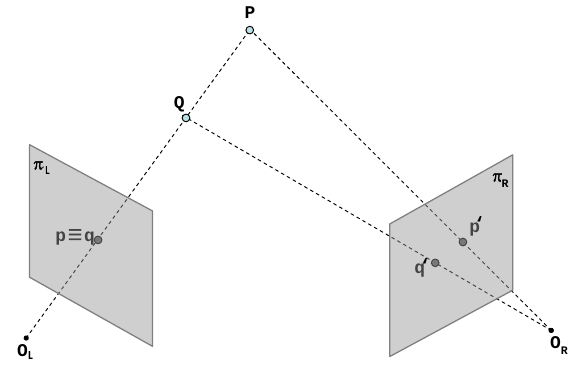
\includegraphics[width=0.6\textwidth]{./img/correspondance.png}
\caption{\scriptsize{Triangulation: with two cameras the depth of }}
\label{fig:corr}
\end{figure}
 The camera setup should be geometrically
calibrated such that the two cameras capture the same part of the real world scene.\\
Calibration of a stereo camera system involves the estimation of the intrinsic and extrinsic parameters of the model: intrinsic parameters embody the characteristics of the optical system and its geometric relationship with the image sensor, extrinsic parameters relate the location and orientation of the second camera with respect to the first one in the 3D space (Figure).\\
\begin{figure}[h!]
\centering
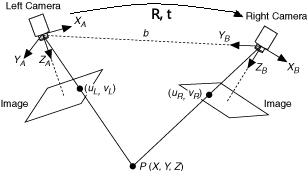
\includegraphics[width=0.6\textwidth]{./img/stereo_system.png}
\caption{\scriptsize{Stereo camera model}}
\label{fig:rt}
\end{figure}
These parameters can be used to rectify a stereo pair of images to make them appear as the two image planes are parallel (Figure). The rectified images are then used to find corresponding points and compute the disparity map.\\
\begin{figure}[h!]
\centering
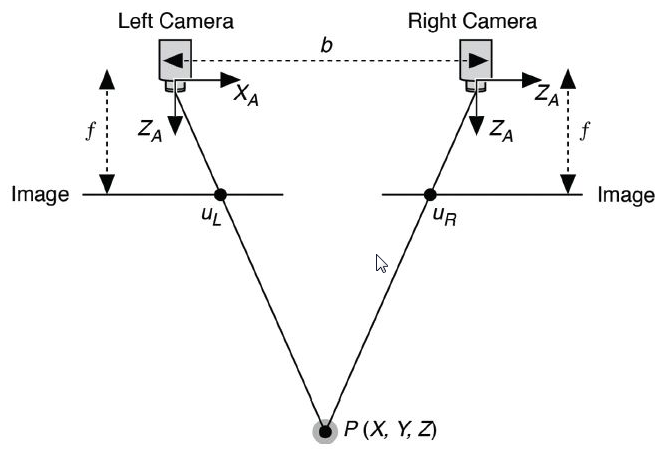
\includegraphics[width=0.6\textwidth]{./img/rect_stereo.png}
\caption{\scriptsize{Rectified stereo cameras}}
\label{fig:rect_stereo}
\end{figure}

\subsection{Disparity map computation}

After the images have been rectify



\section{Acquisition of stereo images}


\section{Display 3D video}
